In this section, a simple and light-weight version of the Resnet version has been implemented, trained and evaluated.
\begin{figure}%
    \centering
    \subfloat[\centering Training loss for Convnet]{{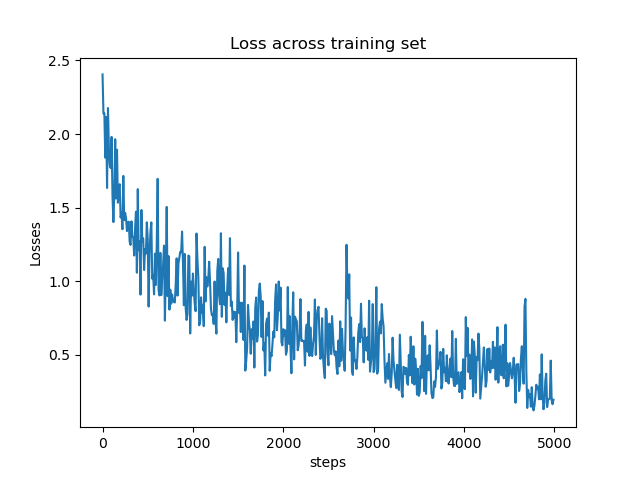
\includegraphics[width=6.5cm]{images/convnet-train_loss.png} }}%
    \qquad
    \subfloat[\centering Test accuracy for Convnet]{{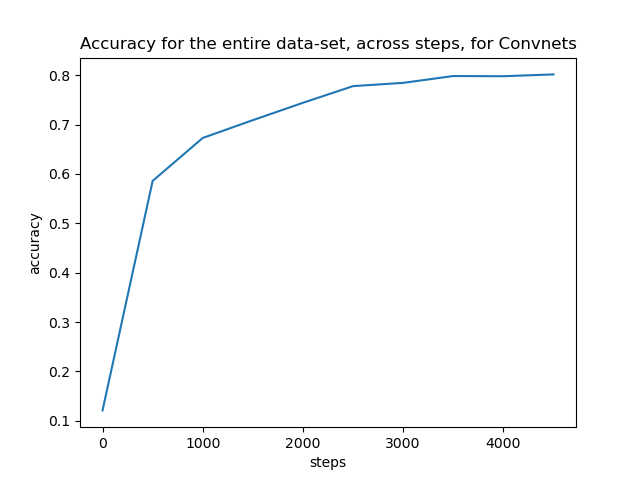
\includegraphics[width=6.5cm]{images/convnet-test_accs.png} }}%
    \caption{Default performance, test and train, for Convnet}%
    \label{fig:defaults}%
\end{figure}

By the end of the default number of steps, the model was not necessarily showing any sign of "stopping". 
What is interesting to note, is that the model seems to reach a point where the accuracy's linear increase (around 800 steps as seen in testing scores)
slopes down a bit. While it does not reach convergence yet, it seems that from this point the model slows down
its learning considerably; this is likely a decrease in learning rate as set by Adam's optimizer.

It is surprising nonetheless how fast this model learns on "limited" data. The gradients are not vanished,
due to the resnet blocks, which means that even the deeper layers get enough of a signal to keep training.

The loss curve here (admittedly, I should have used averaged scores over steps, but time constraints and LISA server errors proved an extra challenge to run on time again)
indicates "hops": around step 700, 1500, 3000, and 4700, the loss make significant "average" drops.